\begin{figure*}
	\begin{tabular}{c c c c c}
	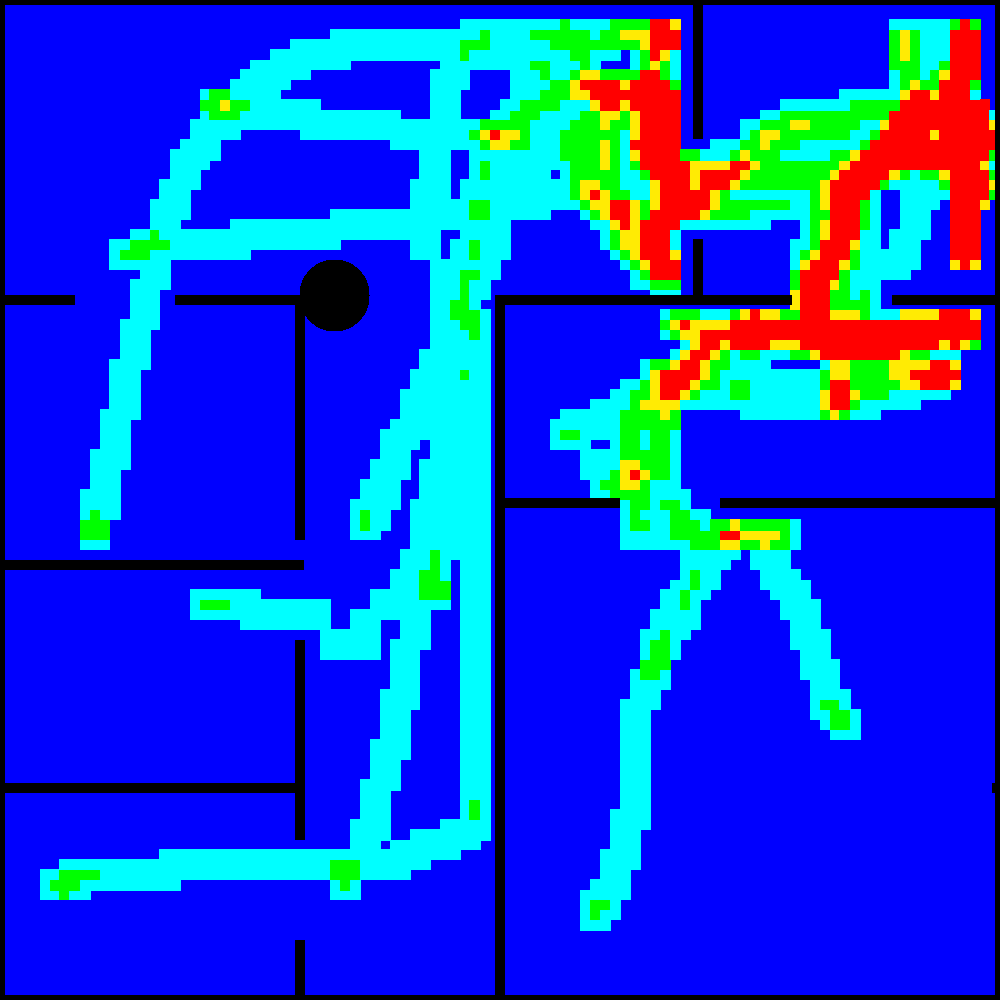
\includegraphics[width=0.19\textwidth]{images/Hypothesis1/Iter1-User-17_t_16_615.png} & 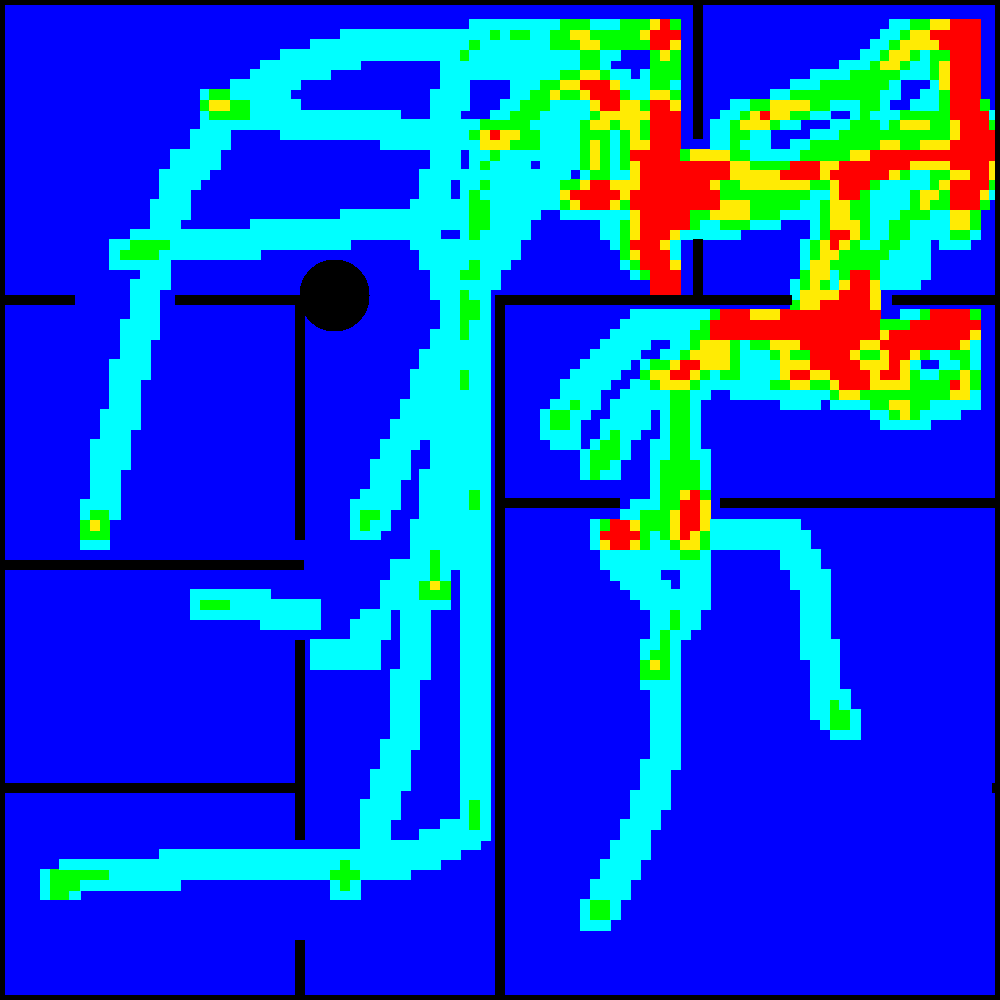
\includegraphics[width=0.19\textwidth]{images/Hypothesis1/Iter2-User-17_t_12_738.png} & 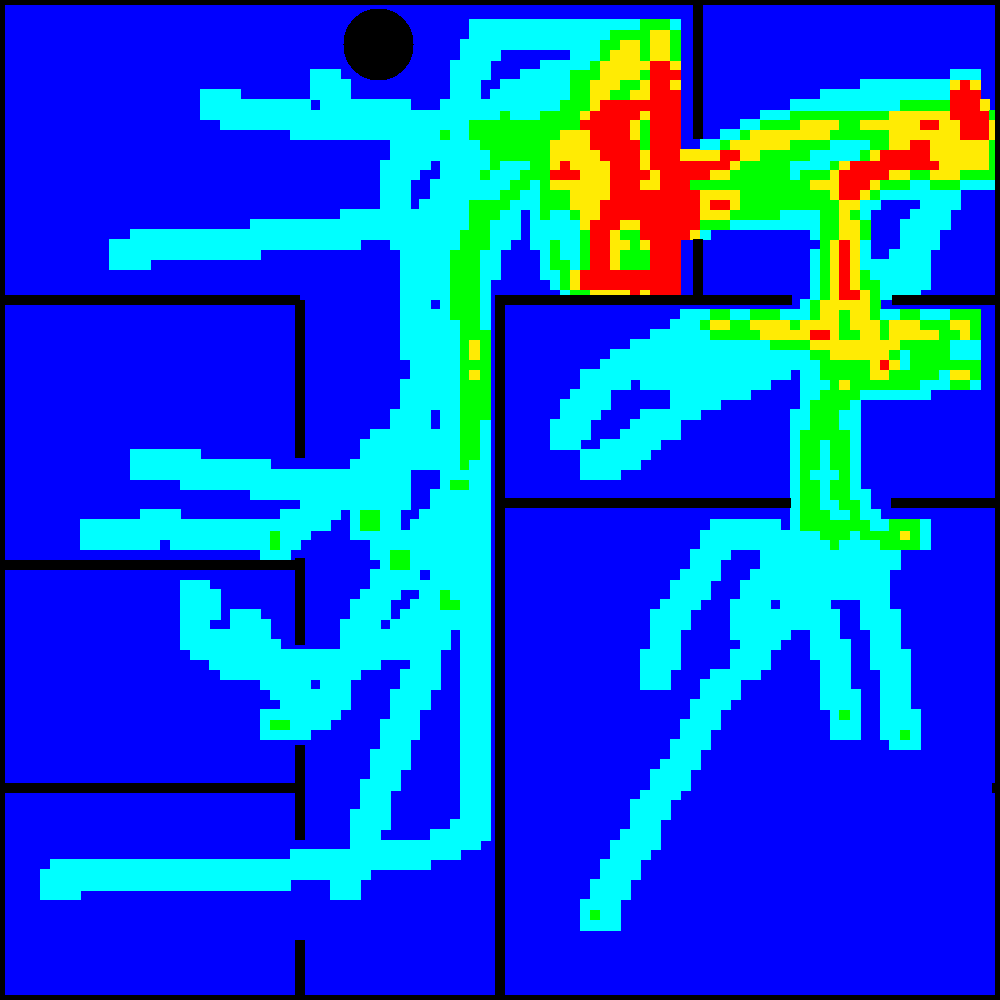
\includegraphics[width=0.19\textwidth]{images/Hypothesis1/Iter3-User-17_t_10_692.png} & 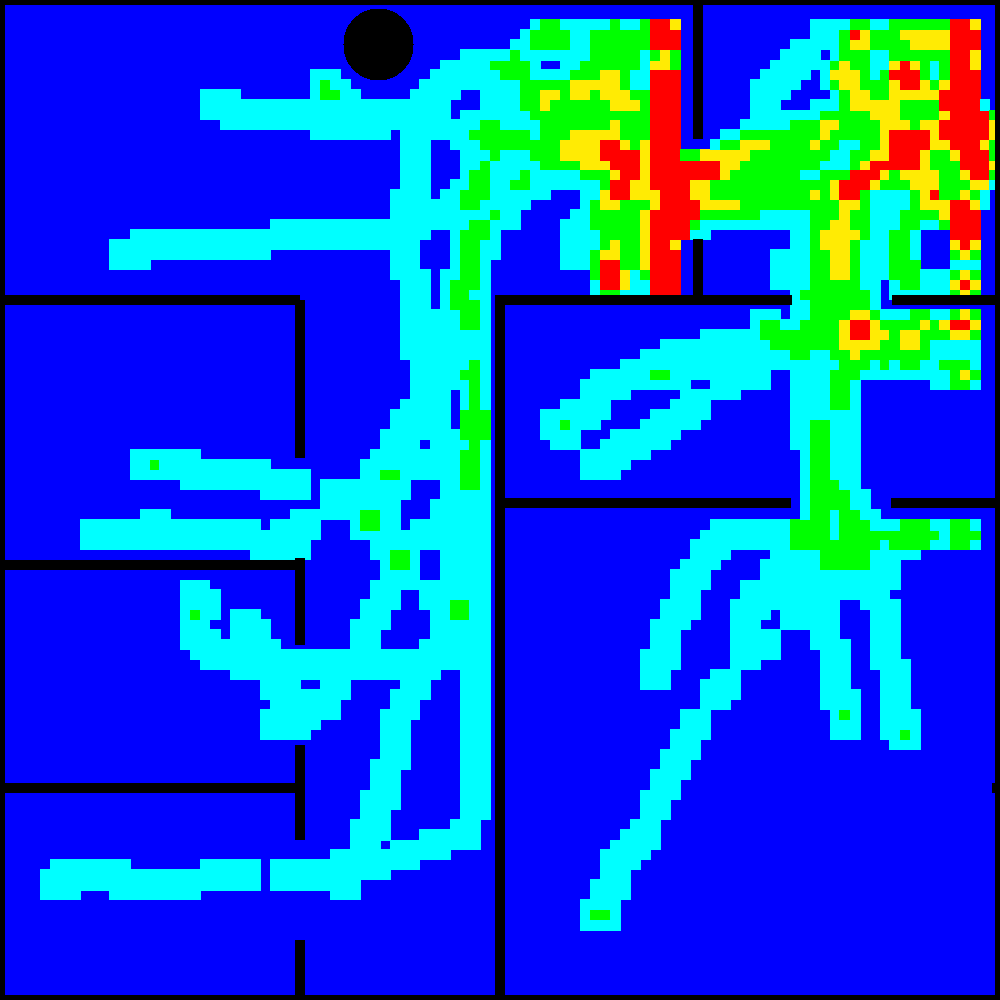
\includegraphics[width=0.19\textwidth]{images/Hypothesis1/Iter4-User-17_t_9_323.png} & 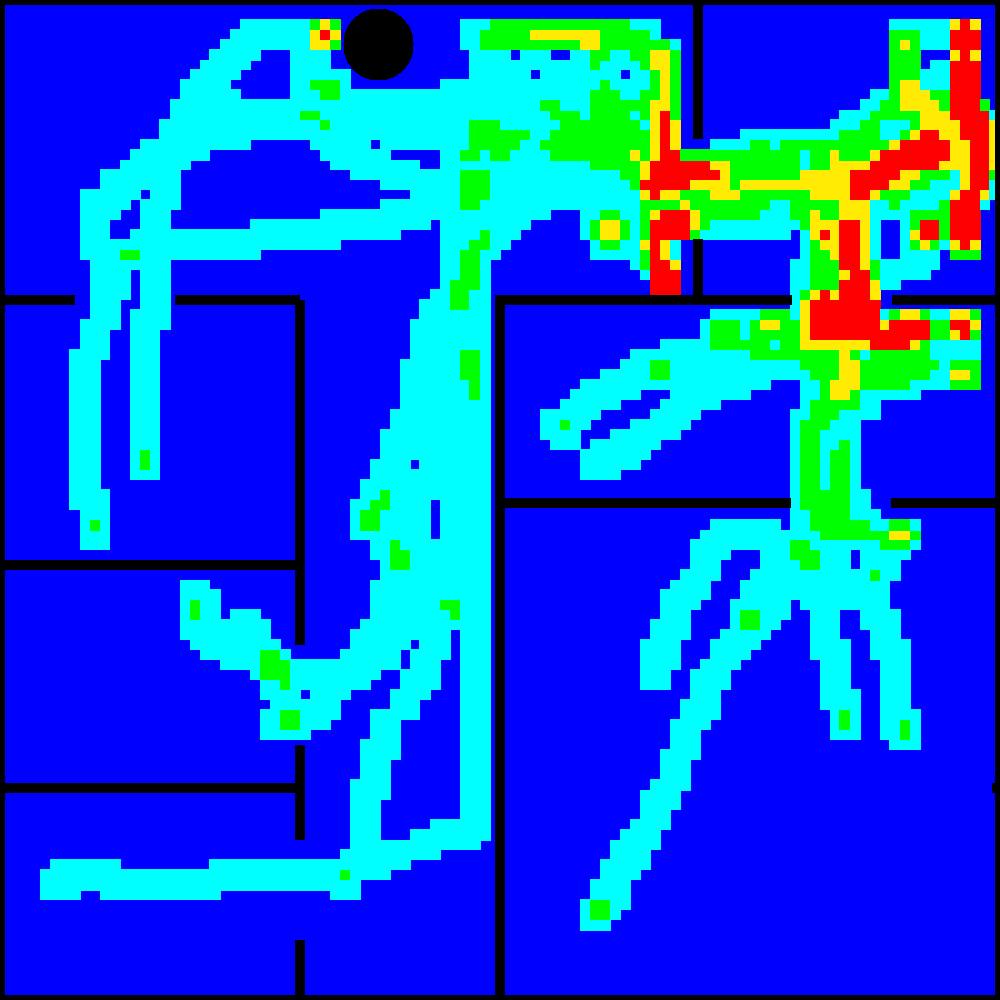
\includegraphics[width=0.19\textwidth]{images/Hypothesis1/Iter5-User-17_t_9_174.png} \\
	(a) & (b) & (c) & (d) & (e)\\
	Time=16.615 & Time= 12.738 & Time=10.692 & Time=9.323 & Time=9.174
	\end{tabular}
	\caption{\label{fig:single-player-iterative-improvement}Iterative environment improvement, in terms of evacuation time, is shown from left to right.}
\end{figure*}

A suite of analysis tools are made available to a player in order to visually validate their simulation results.  In particular we visualize metrics using heatmap so that the user can improve their design by identifying regions which are not performing well. The heat map is an orthographic view of the design containing all the elements(walls, doors,pillars) placed by the user and the path of all the agents. The level of crowd density of a region in the layout can be deduced by different coloured dots in the heat map. Figure~\ref{fig:single-player-iterative-improvement} is an example of a heat map which shows the orthographic view of walls, doors, and pillars in the layout with aggregate crowds dynamics displayed as heat traces. If a region is not performing well, it will become congested and crowd density will rise and the region will become more red. A player can be improve the design to reduce the highlighted areas in the design.


